% [原文 p.121]
\chapter[K 理论中的幂算子]{K 理论中的幂算子\footnotemark}
\footnotetext{M. F. Atiyah, “Power Operations in K-theory”, \textit{Q. J. Math.} \textbf{17} (1) (1966) 165--193.}

\para{引言}

对任意有限 CW 复形 $X$，都可以定义 Grothendieck 群 $K(X)$。$K(X)$ 由 $X$ 上复向量丛的集合构造而成（确切的定义见 [8]）。$K(X)$ 有许多与 $X$ 的上同调形式相似的方面，但有一个决定性的区别。上同调按维数分次，而 $K(X)$ 上只有滤过。这里，子群 $K_q(X)$ 定义为限制同态
\[
  K(X)\longrightarrow K(X_{q-1})
\]
的核，其中 $X_{q-1}$ 是 $X$ 的 $(q-1)$ 维骨架。又，$K(X)$ 带有由向量丛的张量积诱导的环结构，并且它与滤过相容，因此 $K(X)$ 成为带滤过的环。$K(X)$ 上还有由外幂诱导的自然算子。本文的主要目的之一，就是考察算子与滤过之间的关系（定理 B.4.3）。

% [Tutor Note: 这里的 $K_q(X)$ 是滤过的第 $q$ 层，即限制到 $(q-1)$ 维骨架上为零的丛类；下标 $q$ 越大子群越小，与“$q$ 次”的直觉相反。下文 $GK(X)$ 取商 $K_{2q}(X)/K_{2q-1}(X)$，正是要把只有滤过的 $K(X)$ 强行分次化。]

$K(X)$ 与上同调不只是形式相似，二者之间还有更明确的联系。当 $X$ 无挠时，这种联系具有极简单的形式。即，整系数上同调环的偶数维部分
\[
  H^{ev}(X;\Z) = \sum_q H^{2q}(X;\Z)
\]
与分次环
% [原文 p.122]
\[
  GK(X) = \sum_q K_{2q}(X)/K_{2q-1}(X)
\]
自然同构。由于这个同构映射保持环结构，因此自然要问：能否把 K 理论中的算子与上同调中的 Steenrod 算子联系起来？

从这两个理论中算子如何产生来看，无论哪种情形，对称群都起着关键作用。众所周知，引入 Steenrod 算子的一种方法，是利用对称群（及其子群）的上同调（cf. [10]）。另一方面，向量丛的算子本质上来自一般线性群的表示，而对称群在 $GL(n)$ 的不可约表示的构造中的作用当然早已为人所知（cf. [11]）。细究这两种情形便可看出，对称群在两个理论中的用法本质相同。这些算子，乃是 $k$ 次幂映射与对称群 $S_k$ 的作用相结合的结果。

% [Tutor Note: 下文反复出现的“算子”，指的是函子 $K$ 到自身的自然变换：对每个空间 $X$ 给一个映射 $K(X)\to K(X)$，并与拉回相容。这一点在 p.138 才正式写成 $\operatorname{Op}(K)$，此处先借用其意，初读宜先记住“算子 = 自然的 K 群自映射”。]

让我们发展这一观点。仿照 Steenrod，对 $S_k$ 的任意子群 $G$ 引入相应的 K 理论算子。设 $k=p$（$p$ 为素数），$G=\Z/p$ 为 $p$ 阶循环群，则可知由 $\Z/p$ 定义的非平凡算子只有 Adams 算子 $\psi^p$。这提示 $\psi^p$ 与全体 Steenrod 算子 $\sum P^i$ 之间的类似，并且对无挠空间可以得到 $\psi^p$ 与 $P^i$ 的精确关系（定理 B.6.5）。作为副产品，给出算子 $\psi^p$ 相当简单的几何描述（B.2.7）。

用 Chern 特征标把定理 B.6.5 翻译到有理上同调并不困难，因此（对无挠空间）可以重新得到 Adams 的定理 [1]。事实上，本文正是从试图用更直接、更初等的方法导出 Adams 的结果开始的。

本质上的新结果只在于算子与滤过之间的关系，但重新给出 K 理论算子理论的一个自足的说明看来是适当的。假定读者已知 K 理论的标准事实（cf. [8]）与有限群表示论。关于紧 Lie 群的表示，则不作任何假定。

B.1 节列举对称群与张量积的古典理论中相关的事项。

% [原文 p.123]
基本遵循 Schur 的想法（参见 [11, p. 215]），不把重点放在一般线性群 $\operatorname{GL}(n)$ 上，而放在对称群 $S_k$ 上。这是因为在 K 理论中维数 $n$ 颇为麻烦（甚至会变成负的！），而这样做似乎特别合适。于是，以 $R(S_k)$ 为 $S_k$ 的特征标环，引入分次环
\[
  R_* = \sum_k \Hom_\Z\bigl(R(S_k),\Z\bigr)
\]
并相当详细地研究它。所得的式子中至少有一个（命题 B.1.9）大概鲜为人知。B.2 节说明，通过考虑分次向量丛的张量幂，如何定义环同态
\[
  j\colon R_*\longrightarrow \operatorname{Op}(K),
\]
其中 $\operatorname{Op}(K)$ 表示 K 理论算子的集合。然后把 B.1 节得到的关于 $R_*$ 的详细信息应用于 K 理论。

B.3 节涉及 B.2 节所定义的张量幂的“外化”与“相对化”。B.4 节考察算子与滤过之间的关系。B.5 节处理素数阶循环群以及与之相关的算子。B.6 节结合谱序列 $H^*(X;\Z)\Rightarrow K^*(X)$ 简要考察到此为止的算子，特别地得到与 Steenrod 算子的关系。最后，B.7 节把这些翻译到有理上同调，导出 Adams 的结果。

整体说明因引入 $G$ 空间 $X$ 的函子 $K_G(X)$ 而变得相当简单（B.2 节）。它的初等性质我们证明若干，更详细的叙述参见 [4] 与 [9]。

关键的想法——应当关注作用在向量丛复形的 $k$ 次幂上的对称群——本来出自 Grothendieck。而且，关于 K 理论的算子，本文的说明与 Grothendieck 未发表的研究之间有相当的重叠。P. Cartier 与 B. Kostant 曾给予作者非常有益的讨论。

% [原文 p.124]
\section{张量积与对称群}

\takeaway{本节把对称群的表示环 $R(S_k)$ 及其 $\Z$-对偶组织成分次环 $R_*$，用基本元素 $\Delta_{n,k}$ 证明 $R_*$ 经 $\Delta'$ 同构于 $\lim_n\operatorname{Sym}[t_1,\ldots,t_n]$，从而完全确定 $R_*$ 的结构：多项式环、对偶基、幂和等。}

对任意有限群 $G$，用 $R(G)$ 表示由 $G$ 的不可约复表示（的同构类）生成的自由 Abel 群。它关于张量积成为环。把每个不可约表示对应到它的特征标，$R(G)$ 便嵌入 $G$ 上全体复值类函数的环。常常把 $R(G)$ 与这个子环等同，并称为 $G$ 的特征标环。对任意有限群 $G,H$，有自然的同构映射
\[
  R(G)\otimes R(H)\longrightarrow R(G\times H).
\]

现在，设 $S_k$ 为对称群，$\{V_\pi\}$ 为不可约复 $S_k$ 模的完全集。这里 $\pi$ 可以看作 $k$ 的分割，但不使用这一事实。设 $E$ 为复向量空间，$E^{\otimes k}$ 为其 $k$ 次张量幂。群 $S_k$ 自然作用于 $E^{\otimes k}$，给出熟知的分解
\[
  E^{\otimes k}\cong \sum V_\pi\otimes\pi(E),
\]
其中 $\pi(E)=\Hom_{S_k}(V_\pi,E^{\otimes k})$。特别关注两种极端情形。当 $V_\pi$ 为平凡 1 维表示时，$\pi(E)$ 是 $k$ 次对称幂 $\sigma^k(E)$。当 $V_\pi$ 为符号表示时，$\pi(E)$ 是 $k$ 次外幂 $\lambda^k(E)$。$E$ 的自同态映射 $T$ 诱导 $E^{\otimes k}$ 的 $S_k$ 自同态映射 $T^{\otimes k}$，从而诱导 $\pi(E)$ 的自同态映射 $\pi(T)$。设 $T\in \operatorname{GL}(E)$，则 $\pi(E)$ 成为 $\operatorname{GL}(E)$ 的表示空间，这当然是一般线性群不可约表示的经典构造法。然而，就本文的目的而言，这一点并不重要；我们关心的是特征标公式。因此，按如下方式进行。

% [Tutor Note: 上面的分解依据 $S_k$ 的半单性（有限群表示完全可约）：$\pi(E)=\Hom_{S_k}(V_\pi,E^{\otimes k})$ 是 $V_\pi$ 在 $E^{\otimes k}$ 中的重数空间。当 $V_\pi$ 取平凡表示时得对称幂 $\sigma^k$，取符号表示时得外幂 $\lambda^k$，这两个极端情形正是下文挑出来单独研究的。]

设 $E=\C^n$，$T$ 为对角矩阵 $(t_1,\ldots,t_n)$。$T^{\otimes k}$ 的特征值全是由 $t_1,\ldots,t_n$ 构成的 $k$ 次单项式，因此对每个 $\pi$，$\operatorname{Trace}\pi(T)$ 是 $t_1,\ldots,t_n$ 的整系数齐次多项式。此外，对任意置换矩阵 $S$ 有 $\operatorname{Trace}\pi(T)=\operatorname{Trace}\bigl(\pi(S^{-1}TS)\bigr)$，因此 $\operatorname{Trace}\pi(T)$ 是

% [原文 p.125]
$t_1,\ldots,t_n$ 的对称式。以 $[V_\pi]\in R(S_k)$ 表示 $V_\pi$ 的同构类，并用 $\operatorname{Sym}_k[t_1,\ldots,t_n]$ 表示 $k$ 次对称多项式的全体，则定义
\begin{align*}
  \Delta_{n,k} &= \operatorname{Trace}_{S_k}\bigl(T^{\otimes k}\bigr)\\
  &= \sum_\pi \operatorname{Trace}\pi(T)\otimes[V_\pi]
     \in \operatorname{Sym}_k[t_1,\ldots,t_n]\otimes R(S_k).
\end{align*}
把 $R(S_k)$ 看作特征标环，则 $\Delta_{n,k}$ 是由 $t_1,\ldots,t_n$ 与 $g\in S_k$ 的函数 $\operatorname{Trace}\bigl(gT^{\otimes k}\bigr)$ 给出的。表示这个基本元素的方法有好几种，最简单的是下面的命题。

% [Tutor Note: 左端的 $\operatorname{Trace}_{S_k}(T^{\otimes k})$ 并不是线性映射 $T^{\otimes k}$ 的普通迹（那会等于 $\operatorname{Trace}(T)^k$），而是把 $T^{\otimes k}$ 按 $S_k$ 的不可约表示分块后逐块取迹；正因如此它才落在 $\operatorname{Sym}_k\otimes R(S_k)$ 里，并由函数 $g\mapsto\operatorname{Trace}(gT^{\otimes k})$ 唯一决定。]

\begin{proposition*}{B.1.1}
  对 $k$ 的任意分割 $\alpha=(\alpha_1,\ldots,\alpha_r)$，设 $\rho_\alpha\in R(S_k)$ 为由
  \[
    S_\alpha = S_{\alpha_1}\times S_{\alpha_2}\times\cdots\times S_{\alpha_r}
  \]
  的平凡表示诱导的表示，则
  \[
    \Delta = \sum_{\alpha\vdash k} m_\alpha\otimes\rho_\alpha
  \]
  成立。其中 $m_\alpha$ 是由 $t_1^{\alpha_1}t_2^{\alpha_2}\cdots t_r^{\alpha_r}$ 生成的单项对称函数，求和遍历 $k$ 的所有分割。
\end{proposition*}

\begin{proof}
  设 $E^\alpha$ 为对应于特征值 $t_1^{\alpha_1}t_2^{\alpha_2}\cdots t_r^{\alpha_r}$ 的 $T^{\otimes k}$ 的特征空间。它以向量
  \[
    e_\alpha = e_1^{\otimes\alpha_1}\otimes e_2^{\otimes\alpha_2}\otimes\cdots\otimes e_r^{\otimes\alpha_r}
  \]
  在 $S_k$ 下的轨道为基。其中 $e_1,\ldots,e_n$ 是 $\C^n$ 的标准基。$e_\alpha$ 的固定子群恰好是子群 $S_\alpha$，因此可得 $E^\alpha$ 是诱导表示 $\rho_\alpha$。若 $\alpha$ 与 $\beta$ 是 $k$ 的同一分割，则 $S_\alpha$ 与 $S_\beta$ 共轭，于是导出
  \[
    \Delta = \sum_{|\alpha|=k} t^\alpha\otimes\rho_\alpha
           = \sum_{\alpha\vdash k} m_\alpha\otimes\rho_\alpha.
  \]
  其中第一个求和遍历满足
  \[
    |\alpha| = \sum \alpha_i = k
  \]
  的所有列 $\alpha_1,\alpha_2,\ldots$。
\end{proof}

% [原文 p.126]
这里引入对偶群
\[
  R_*(S_k) = \Hom_\Z\bigl(R(S_k),\Z\bigr).
\]
此时，$\Delta_{n,k}$ 定义了同态映射
\[
  \Delta'_{n,k}\colon R_*(S_k)\longrightarrow \operatorname{Sym}_k[t_1,\ldots,t_n]
\]
（反过来，$\Delta_{n,k}$ 也由这个同态映射定义）。由包含映射
\[
  S_k\times S_l\longrightarrow S_{k+l}
\]
得到同态映射
\[
  R(S_{k+l})\longrightarrow R(S_k\times S_l)
  \cong R(S_k)\otimes R(S_l),
\]
再由对偶性得到
\[
  R_*(S_k)\otimes R_*(S_l)\longrightarrow R_*(S_{k+l}).
\]
设 $R_*=\sum_{k\ge 0}R_*(S_k)$，则关于这个积 $\otimes$，$R_*$ 成为分次交换环。这一点由 $\alpha$ 与 $\beta$ 是同一分割时 $S_\alpha$ 与 $S_\beta$ 共轭可知，该事实在命题 B.1.1 中已经用过。进一步，由 $\Delta'_n=\sum_k\Delta'_{n,k}$ 定义
\[
  \Delta'_n\colon R_*\longrightarrow \operatorname{Sym}[t_1,\ldots,t_n],
\]
则可知 $\Delta'_n$ 是环同态映射。这由迹的乘法性可得。即，设 $g_1\in S_k$，$g_2\in S_l$，则
\[
  \operatorname{Trace}\bigl(g_1g_2T^{\otimes(k+l)}\bigr)
  = \operatorname{Trace}\bigl(g_1T^{\otimes k}\bigr)
    \operatorname{Trace}\bigl(g_2T^{\otimes l}\bigr).
\]
最后，注意交换图表

% [原文 p.127]
\[
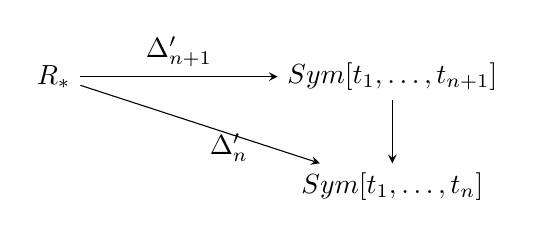
\begin{tikzpicture}[baseline=(current bounding box.center),>=stealth]
  \node (A) at (0,0) {$R_*$};
  \node (B) at (4.3,0) {$\operatorname{Sym}[t_1,\ldots,t_{n+1}]$};
  \node (C) at (4.3,-1.4) {$\operatorname{Sym}[t_1,\ldots,t_n]$};
  \draw[->] (A) -- node[above] {$\Delta'_{n+1}$} (B);
  \draw[->] (A) -- node[below right] {$\Delta'_n$} (C);
  \draw[->] (B) -- (C);
\end{tikzpicture}
\]
其中向下的箭头由令 $t_{n+1}=0$ 给出。因此，取极限可得
\[
  \Delta'\colon R_*\longrightarrow \lim_n \operatorname{Sym}[t_1,\ldots,t_n].
\]
这里，射影极限是在分次环的范畴中取的，故
\[
  \lim_n \operatorname{Sym}[t_1,\ldots,t_n]
  = \sum_{k=0}^\infty \lim_n \operatorname{Sym}_k[t_1,\ldots,t_n]
\]
是齐次部分的（不是直积的）直和。

\begin{proposition*}{B.1.2}
  \[
    \Delta'\colon R_*\longrightarrow \lim_n \operatorname{Sym}[t_1,\ldots,t_n]
  \]
  是同构映射。
\end{proposition*}

\begin{proof}
  用 $\sigma^k\in R_*(S_k)$ 表示由
  \[
    \sigma^k(1)=1,\qquad
    V_\pi\neq 1\ \text{时}\ \sigma^k(V_\pi)=0
  \]
  定义的同态 $R(S_k)\to\Z$。其中 $1$ 表示平凡表示。$V_\pi=1$ 时 $\pi(E)$ 是 $E$ 的 $k$ 次对称幂，所以由 $\Delta'_{n,k}$ 的定义可导出
  \[
    \Delta'_{n,k}(\sigma^k) = h_k(t_1,\ldots,t_n)
  \]
  是 $k$ 次齐次对称函数（即 $\prod(1-zt_i)^{-1}$ 中 $z^k$ 的系数）。由于 $h_k$ 构成对称函数的多项式基，可知 $\Delta'_n$ 对所有 $n$ 都是满射同态。现在，$R(S_k)$ 的秩等于 $S_k$ 的共轭类个数，即
  % [原文 p.128]
  $k$ 的分割的个数，从而当 $n\ge k$ 时也等于 $\operatorname{Sym}_k[t_1,\ldots,t_n]$ 的秩。于是，
  \[
    \Delta'_{n,k}\colon R_*(S_k)\longrightarrow \operatorname{Sym}_k[t_1,\ldots,t_n]
  \]
  对 $n\ge k$ 是秩相同的自由交换群之间的满射同态，因此是同构映射。对 $n\ge k$，
  \[
    \operatorname{Sym}_k[t_1,\ldots,t_{n+1}]
    \longrightarrow \operatorname{Sym}_k[t_1,\ldots,t_n]
  \]
  也是同构映射，故证明完成。
\end{proof}

% [Tutor Note: 证明的关键是秩的比对：$\operatorname{Sym}_k[t_1,\ldots,t_n]$ 的秩等于 $k$ 的分割数，$R_*(S_k)$ 的秩等于 $S_k$ 的共轭类数，而 $S_k$ 的共轭类与 $k$ 的分割一一对应。先证满射、再证秩相等，即得同构；这是有限自由交换群证明同构的常用套路。]

\begin{corollary*}{B.1.3}
  $R_*$ 是由 $\sigma^1,\sigma^2,\ldots$ 生成的多项式环。
\end{corollary*}

代替元素 $\sigma^k\in R_*(S_k)$，用由
\[
  \lambda^k(V_\pi)=
  \begin{cases}
    1 & (V_\pi\ \text{为符号表示时}),\\
    0 & (\text{其他情形})
  \end{cases}
\]
定义的元素 $\lambda^k$ 也可以做同样的事。当 $\pi$ 是 $S_k$ 的符号表示时，$\pi(E)$ 是 $k$ 次外幂，因此可导出
\[
  \Delta'_{n,k}(\lambda^k) = e_k(t_1,\ldots,t_n)
\]
是 $k$ 次基本对称函数。因此，$R_*$ 也是以 $\lambda^1,\lambda^2,\ldots$ 为生成元的多项式环。

\begin{corollary*}{B.1.4}
  设 $\Delta_{n,k}=\sum a_i\otimes b_i$ 中的 $a_i\in\operatorname{Sym}_k[t_1,\ldots,t_n]$、$b_i\in R(S_k)$，且 $n\ge k$。此时，$a_i$ 构成基与 $b_i$ 构成基等价。当这成立时，$a_i$ 决定 $b_i$，$b_i$ 也决定 $a_i$。即，它们互为“对偶基”。
\end{corollary*}

\begin{proof}
  把 $\Delta'_{n,k}$ 是同构映射这一事实重新解释，即可立即导出。
\end{proof}

\begin{corollary*}{B.1.5}
  表示 $\rho_\alpha\ (\alpha\vdash k)$ 构成 $R(S_k)$ 的基。
\end{corollary*}

% [原文 p.129]
\begin{proof}
  对命题 B.1.1 给出的 $\Delta_{n,k}$ 的式子应用推论 B.1.4。由于 $m_\alpha$ 是对称函数的基，可知 $\rho_\alpha$ 构成 $R(S_k)$ 的基。
\end{proof}

\begin{corollary*}{B.1.6}
  $S_k$ 的特征标对所有共轭类取整数值。
\end{corollary*}

\begin{proof}
  所有 $\rho_\alpha$ 的特征标都取整数值，因此推论 B.1.6 由推论 B.1.5 导出。
\end{proof}

\para{附记.}
当然，推论 B.1.6 也可以从别的论证简单导出。

用 $C(S_k)$ 表示 $S_k$ 上整值类函数的群。由推论 B.1.6，有自然的同态映射
\[
  R(S_k)\longrightarrow C(S_k).
\]
这个映射的核为零，余核有限。因此，对偶同态映射
\[
  C_*(S_k)\longrightarrow R_*(S_k)
\]
也有同样的事实。直和 $C_*=\sum_{k\ge 0}C_*(S_k)$ 具有自然的环结构，
\[
  C_*\longrightarrow R_*
\]
是环同态映射。把 $C_*$ 与它在 $R_*$ 中的像所成的子环等同。由定义，$C_*(S_k)$ 是 $S_k$ 的共轭类上的自由 Abel 群。用 $\psi^k$ 表示长度 $k$ 的循环置换的共轭类。此时，$C_*$ 是 $\psi^1,\psi^2,\ldots$ 上的多项式环。下面的结果决定由对称函数组成的子环 $\Delta'(C_*)$。

\begin{proposition*}{B.1.7}
  $\Delta'_n(\psi^k)=m_k(t_1,\ldots,t_n)=\sum_{i=1}^n t_i^k$，因此 $\Delta'(C_*)$ 是由幂和 $m_k$ 生成的子环。
\end{proposition*}

\begin{proof}
  设 $g\in S_k$ 为长度 $k$ 的循环置换，则由定义
  \[
    \Delta'_n(\psi^k) = \operatorname{Trace}\bigl(gT^{\otimes k}\bigr).
  \]
  这里，用命题 B.1.1 计算这个迹，便得
  % [原文 p.130]
  \[
    \Delta'_n\psi^k = \sum_{\alpha\vdash k} m_\alpha\rho_\alpha(g).
  \]
  然而，当 $H\subset G$ 时，由 $H$ 诱导到 $G$ 的特征标，对与 $H$ 的元素在 $G$ 中不共轭的元素取零。因此，令 $H=S_\alpha$，$G=S_k$，可知只要 $\alpha=k$（即 $\alpha$ 单独构成 $k$ 的分割）不成立，就有 $\rho_\alpha(g)=0$。由于 $\rho_k(g)=1$，可得
  \[
    \Delta'_n\psi^k = m_k.
  \]
\end{proof}

\begin{corollary*}{B.1.8}
  设 $Q_k$ 为用基本对称式 $e_1,\ldots,e_k$ 表示幂和 $m_k$ 的牛顿多项式。即设
  \[
    m_k = Q_k(e_1,\ldots,e_k).
  \]
  此时，
  \[
    \psi^k = Q_k(\lambda^1,\ldots,\lambda^k)\in R_*
  \]
  成立。
\end{corollary*}

\para{注.}
考虑与有理数域 $\Q$ 的张量积，可引入由分割 $\alpha$ 定义的共轭类的特征函数
\[
  \varepsilon_\alpha\in R(S_k)\otimes\Q.
\]
此时，命题 B.1.7 本质上与下面的 $\Delta_{n,k}$ 的式子等价（cf. [11, VII (7.6)]）。
\[
  \Delta_{n,k} = \sum_{\alpha\vdash k} p_\alpha(t)\otimes\varepsilon_\alpha
  \in \operatorname{Sym}_k[t_1,\ldots,t_n]\otimes R(S_k)\otimes\Q,
\]
其中 $p_\alpha$ 是由幂和构成的单项式
\[
  p_\alpha = \prod_{i=1}^k (m_i)^{\alpha_i},\qquad
  \alpha = 1^{\alpha_1}2^{\alpha_2}\cdots.
\]
由于 $\Delta'(\lambda^k)=e_k$，所以 $\Delta_{n,k}$ 可以写成

% [原文 p.131]
\[
  \Delta_{n,k} = \sum_{\alpha\vdash k} q_\alpha(t)\otimes b_\alpha.
\]
其中 $q_\alpha$ 是由基本对称式构成的单项式
\[
  q_\alpha = \prod_{i=1}^k (e_i)^{\alpha_i},\qquad
  \alpha = 1^{\alpha_1}2^{\alpha_2}\cdots.
\]
而 $b_\alpha$ 是 $R(S_k)$ 中唯一确定的某个元素。一般不去求 $b_\alpha$，但下面的命题给出“最高次系数”$b_k$。

\begin{proposition*}{B.1.9}
  用 $M$ 表示 $S_k$ 的 $(k-1)$ 维表示，它由标准 $k$ 维表示的子空间 $\sum_{i=1}^k z_i=0$ 给出。设 $\Lambda^i(M)$ 为 $M$ 的 $i$ 次外幂，
  \[
    \Lambda_{-1}(M) = \sum (-1)^i\Lambda^i(M)\in R(S_k).
  \]
  此时，
  \[
    \Delta_{n,k} = (-1)^{k-1}e_k(t)\otimes\Lambda_{-1}(M) + \text{复合项}
  \]
  成立，其中“复合”意味着至少含有两个 $e_i(t)$ 的乘积。
\end{proposition*}

\begin{proof}
  在式
  \[
    \Delta_{n,k} = \sum_{\alpha\vdash k} q_\alpha(t)\otimes b_\alpha
  \]
  中，$b_\alpha$ 是 $R(S_k)$ 的基，且为 $\lambda^i$ 的单项式所构成的 $R_*(S_k)$ 的基的对偶。因此，$b_k$ 由条件
  \begin{gather*}
    \langle b_k,\lambda^k\rangle = 1,\\
    \langle b_k,u\rangle = 0\qquad
    (u\ \text{是}\ \lambda^i\ \text{的复合的情形})
  \end{gather*}
  定义。$\psi^i$ 与 $\lambda^i$ 由推论 B.1.8 的等式联系起来：
  \[
    \psi^k = Q_k(\lambda^1,\ldots,\lambda^k)
    = (-1)^{k-1}k\lambda_k + \text{复合项},
  \]
  所以 $b_k$ 也可以由条件
  % [原文 p.132]
  \begin{gather*}
    \langle b_k,\psi^k\rangle = (-1)^{k-1}k,\\
    \langle b_k,u\rangle = 0\qquad
    (u\ \text{是}\ \psi^i\ \text{的复合的情形})
  \end{gather*}
  定义。为了证明 $b_k=(-1)^{k-1}\Lambda_{-1}(M)$，还须确认特征标 $\Lambda_{-1}(M)$ 在所有复合类上消失，而在长度 $k$ 的循环置换上取值 $k$。现在，若 $g\in S_k$ 是循环置换的乘积，即不是长度 $k$ 的循环置换，则它作用在 $M$ 上时以 $1$ 为特征值。设其循环置换分解为 $g=(1\ \cdots\ r)(r+1\ \cdots\ s)\cdots$，则其特征向量由
  \[
    z_i=\frac{1}{r}\ (1\le i\le r),\qquad
    z_j=-\frac{1}{k-r}\ (j>r)
  \]
  给出。设 $g_M$ 为 $g$ 所定义的 $M$ 的线性变换，则 $\Lambda_{-1}(M)(g)=\det(1-g_M)$，所以 $g_M$ 以 $1$ 为特征值意味着 $\Lambda_{-1}(M)(g)=0$。最后，取 $g=(1\ 2\ \cdots\ k)$，考虑 $k$ 维表示 $N=M\oplus 1$。此时，$g_N$ 由矩阵
  \[
    g_N=
    \begin{pmatrix}
      0 & 1 &   &        &   \\
        & 0 & 1 &        &   \\
        &   & \ddots & \ddots &   \\
        &   &   & \ddots & 1 \\
      1 &   &   &        & 0
    \end{pmatrix}
  \]
  给出。因此，$\det(1-tg_N)=1-t^k$。于是，
  \begin{align*}
    \det(1-tg_M) &= \det(1-tg_N)\cdot(1-t)^{-1}\\
    &= \frac{1-t^k}{1-t} = 1+t+t^2+\cdots+t^{k-1},
  \end{align*}
  并且
  \[
    \Lambda_{-1}(M)(g) = \det(1-g_M) = k
  \]
  成立。
\end{proof}

% [Tutor Note: 原书 p.131 的式子 $\psi^k=Q_k(\lambda^1,\ldots,\lambda^k)=(-1)^{k-1}k\lambda_k+$ 复合项 把 $\lambda$ 写成下标 $\lambda_k$，与本节其余各处的外幂 $\lambda^k$（上标）不一致；按牛顿恒等式，此处应为 $(-1)^{k-1}k\lambda^k$，疑为笔误。]

% [Tutor Note: 等式 $\Lambda_{-1}(M)(g)=\det(1-g_M)$ 来自外幂的特征标公式：$\sum_i(-1)^i\operatorname{Trace}\Lambda^i(g_0)=\det(1-g_0)$。因此 $g_M$ 有特征值 1 时右边为零，这正是“$\Lambda_{-1}(M)$ 在复合类上消失”的依据；而在长度 $k$ 的循环置换上，$M$ 的特征值为除 1 以外的全部 $k$ 次单位根，故 $\prod_{i=1}^{k-1}(1-\zeta^i)=k$。]

% 块尾跨页句：であり、Λ_{-1}(M)(g)=det(1-g_M)=k が成り立つ。（原书 p.132 末行起句，续至 p.133 首行，已并入本块）

% CHUNK appB1 DONE
